\documentclass[DaoFP]{subfiles}
\begin{document}
\setcounter{chapter}{10}

\chapter{Dependent Types}

A family of types parameterized by a set.

Can be seen as a type with a projection

Fiber times base

Slice categories or over categories

C/B: objects E/B are bundles

morphisms preserve fibers

generalize fiber bundles

base-change functor

pullback 


locally closed categories

pullback to a terminal-object base picks a fiber

relation to logic: universal/esistential quantification

equality types

\section{Dependent Sum}

sigma type

a pair, but the type of the second component depends on the value of the first

as fibration 

\[
 \begin{tikzcd}
 G
 \arrow[dr, dashed, "\phi^T"]
 \arrow[drr, bend left, "\phi"]
 \arrow[ddr, bend right, "q"]
 \\
 &B \times E
 \arrow[r, "\pi_2"]
 \arrow[d, "\pi_1"']
 &E
 \arrow[d, "!"]
 \\
 &B
 \arrow[r, "!"]
 &1
  \end{tikzcd}
\]

\[(\mathcal{C}/B)(\langle G, q \rangle, \langle B \times E, \pi_1 \rangle) \cong \mathcal{C}(G, E) \]

\[
 \begin{tikzcd}
 G
 \arrow[dr, dashed, "\phi^T"]
 \arrow[drr, bend left, "\phi"]
 \arrow[ddr, bend right, "q"]
 \\
 &G'
 \arrow[r, "g"]
 \arrow[d, "f^* p"']
 &E
 \arrow[d, "p"]
 \\
 &B
 \arrow[r, "f"]
 &B'
  \end{tikzcd}
\]

\[  (\mathcal{C}/B) (\langle G, q \rangle , \langle G', f^* p\rangle ) \cong (\mathcal{C}/B') \big(\langle G, \Sigma_f q\rangle , \langle E, p\rangle \big) \]
\[
\begin{tikzcd}
 G
 \arrow[rr, "\phi^T"]
 \arrow[rd, "q"']
 && G'
 \arrow[ld, "f^* p"]
 \\
 & B
  \end{tikzcd}
 \hspace{20pt}
 \begin{tikzcd}
 G
 \arrow[rr, "\phi"]
 \arrow[rd, "\Sigma_f q"']
 &&E
 \arrow[dl, "p"]
 \\
 &B'
  \end{tikzcd}
\]

\[ \Sigma_f q = f \circ q \]




left adjoint to base-change functor

proof by universal property of pullbacks

terminal-object base picks a fiber

terminal-object as bundle over termina-object base: picks en element of a given fiber


\section{Dependent Product}

\[
 \begin{tikzcd}
 G \times B
 \arrow[d, "\phi^T \times B"']
 \arrow[dr, "\phi"]
 \\
 S \times B
 \arrow[r, "\varepsilon"]
 &E
  \end{tikzcd}
\]


Bundle $E/B$ (can be thought of as a sum of fibres).

Family of sections $S$ of a bundle $E$ over $B$. Equipped with a projection $p \colon E \to B$.

Evaluation map $\varepsilon \colon S \times B \to E$ must commute with projection, so it's an arrow in $\mathbf{Set}/B$.

Universal property: For any other set $G$ and a mapping in $\mathbf{Set}/B$,  $\phi \colon G \times B \to E$, there is a unique mapping $\phi^T \colon G \to S$ that makes things commute.

\[\mathbf{Set} (G, S) \cong (\mathbf{Set}/B)(\langle G\times B, \pi_2\rangle , \langle E, p\rangle ) \]
\[\pi_2 \colon G \times B \to B \]
\[p \colon E \to B \]

this can be written as:

\[(\mathbf{Set}/1) (\langle G, !\rangle , \langle S, !\rangle ) \cong (\mathbf{Set}/B)(\langle G\times B, \pi_2\rangle , \langle E, p\rangle )  \]

$G \times B$ is a pullback from the terminal object
\[
 \begin{tikzcd}
 G \times B
 \arrow[d, "\pi_2"]
 \arrow[r, "\pi_1"]
 & G
 \arrow[d, "!"]
 \\
 B
 \arrow[r, "!"]
 &
 1
  \end{tikzcd}
\]

Given $f \colon B \to B'$, we have the base-changer functor $f^* \colon \mathcal{C}/B' \to \mathcal{C}/B$.

$\Pi_f \colon \mathcal{C}/B \to \mathcal{C}/B'$ is right adjoint to $f^*$

\[(\mathcal{C}/B')(\langle G, q \rangle, \langle S, \Pi_f \,p\rangle) \cong (\mathcal{C}/B) (\langle G', f^* q\rangle, \langle E, p \rangle) \]

\[
\begin{tikzcd}
 G
 \arrow[rr, "\phi^T"]
 \arrow[rd, "q"']
 && S
 \arrow[ld, "\Pi_f \, p"]
 \\
 & B'
  \end{tikzcd}
 \hspace{20pt}
 \begin{tikzcd}
 G'
 \arrow[rr, "\phi"]
 \arrow[rd, "f^* q"']
 &&E
 \arrow[dl, "p"]
 \\
 &B
  \end{tikzcd}
\]

\[
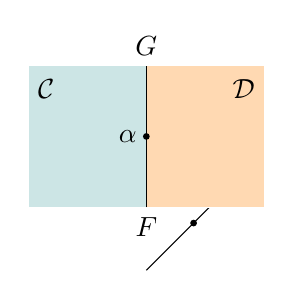
\begin{tikzpicture}
\def\dy{0.6};
\def\ybl{0}; % base left
\def\ybm{\dy}; % base middle
\def\ybr{2*\dy}; % base right

\def\dx{0.6};
\def\xbl{0};
\def\xbm{\dx};
\def\xbr{2*\dx};

\draw (\xbl, \ybl) -- (\xbr, \ybr);
\filldraw[black] (\xbm, \ybm) circle (1 pt);



\def\x{0};
\def\xl{-1.5};
\def\xr{1.5};


\def \ya{0.8};
\def \yb{1.7};
\def \yc{2.6};
\def \yt {2.3};

\filldraw[fill=blue!50!green!20, draw=white] (\xl, \ya) rectangle (\x, \yc);
\filldraw[fill=orange!30, draw=white] (\x, \ya) rectangle (\xr, \yc);

\node[below] (a) at (\x, \ya) {$F$};
\node(b) at (\x, \yb) {};
\node [above] (c) at (\x, \yc) {$G$};

\node(l)[right] at (\xl, \yt) {$\mathcal{C}$};
\node(r)[left] at (\xr, \yt) {$\mathcal{D}$};


\filldraw[black] (b) circle (1 pt);
\node [left] at (b) {$\alpha$};

\draw (a)  -- (c);

\end{tikzpicture}
\]

\subsection{notes}


\begin{exercise}
\end{exercise}

\begin{haskell}
\end{haskell}

\[
 \begin{tikzcd}
  \end{tikzcd}
\]

\[   \mathbf{Set} \]
\[   \mathcal{C} \]

\end{document}